\documentclass{beamer}
\usetheme{AnnArbor}
\usecolortheme{beaver}
\usepackage{tikz}
\usepackage{color}
\usepackage{listings}

\lstset{language=Java,
  basicstyle=\footnotesize\ttfamily,
  keywordstyle=\footnotesize\color{blue}\ttfamily,
  commentstyle=\footnotesize\color{gray}\ttfamily,
}

\definecolor{darkred}{rgb}{0.8,0,0}

\setbeamercolor{title}{fg=white,bg=darkred!80!black}
\setbeamercolor{frametitle}{fg=darkred!80!black,bg=white}
%\setbeamercolor{section in head/foot}{fg=green,bg=yellow}
%\setbeamercolor{subsection in head/foot}{bg=white}
\begin{document}
\title{Functional Testing with RedDeer}   
\author{Andrej Podhradsky}
\date{\today} 
%\logo{
\includegraphics[height=1cm]{reddeer_logo.png}\vspace{220pt}}

\addtobeamertemplate{title page}{\center{
\includegraphics[height=2cm]{reddeer_logo.png}}}{}

\addtobeamertemplate{frametitle}{}{
\begin{tikzpicture}[remember picture,overlay]
\node[anchor=north east,yshift=-8pt] at (current page.north east) {
\includegraphics[height=1cm]{reddeer_logo.png}};
\end{tikzpicture}}

\frame{\titlepage} 

% \frame{\frametitle{Table of contents}\tableofcontents} 

\section{Introduction}

\subsection{Example}
\begin{frame}[fragile]
\begin{center}
\frame{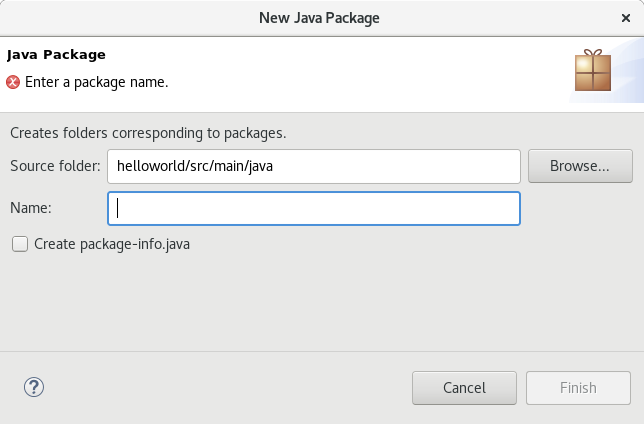
\includegraphics[width=\textwidth,height=0.8\textheight,keepaspectratio]{new_java_package.png}}
\end{center}
\end{frame}

\begin{frame}[fragile]
\begin{lstlisting}
@RunWith(RedDeerSuite.class)
public class NewPackageWizardTest {
  ...
\end{lstlisting}
\pause
\begin{lstlisting}
  @Test
  public void testCreatingNewJavaPackage() {    
    Shell = new DefaultShell("New Java Package");
    new LabeledText(shell, "Name:").setText("helloworld");
    new PushButton(shell, "Finish").click();
\end{lstlisting}
\pause
\begin{lstlisting}
    new WaitWhile(new ShellIsAvailable(shell));
\end{lstlisting}
\end{frame}

%\subsection{About RedDeer}
%\begin{frame}[fragile]
%\frametitle{About RedDeer}
%An extensible framework used for development of automated SWT/Eclipse tests which
%\begin{itemize}
%\item interacts with application’s user interface
%\item uses a programmatic approach just like SWTBot
%\item can be executed from IDE and from command line
%\end{itemize}
%\end{frame}

\subsection{RedDeer vs SWTBot}
\begin{frame}[fragile]
\frametitle{RedDeer vs SWTBot}
RedDeer  
\begin{lstlisting}
new PushButton("OK").click();
new LabeledText("Projec name").setText("helloworld");
new TextEditor("Demo.java").save();
\end{lstlisting}
\vspace{0.5cm}
SWTBot
\begin{lstlisting}
bot.button("OK").click();
bot.textWithLabel("Project name").setText("helloworld");
bot.editor("Demo.java").save();
\end{lstlisting}
\end{frame}

\begin{frame}[fragile]
\frametitle{RedDeer vs SWTBot}
Common features in RedDeer and SWTBot
\begin{itemize}
\item Works with SWT, Eclipse plugins and RCP applications
\item Supports Windows, Macosx and Linux
\item Uses tycho for building plugins with maven
\item Tests are executed in a non-UI thread
\item Uses matchers from hamcrest lib for finding widgets
\item Screenshot is captured if an exception is thrown
\item GEF support
\end{itemize}
\end{frame}

\begin{frame}[fragile]
\frametitle{RedDeer vs SWTBot}
RedDeer
\begin{itemize}
\item Hi-Level API - wizards, views from JEE
\item Enhanced waiting conditions
\item Requirements
\item Basic Graphiti support
\end{itemize}
\vspace{0.5cm}
SWTBot
\begin{itemize}
\item e4 support
\end{itemize}
\end{frame}

\section{RedDeer in Details}

\subsection{Finding a widget}
\begin{frame}[fragile]
\frametitle{Hamcrest matchers}
\begin{lstlisting}
public class MyMatcher extends BaseMatcher {

  private String text;

  public MyMatcher(String text) {
    this.text = text;
  }
  
  @Override
  public boolean matches(Object object);
    if (object instance of Button) {
      return ((Button) object).getText().equals(text);
    }
  }

} 
\end{lstlisting}
\end{frame}

\begin{frame}[fragile]
\frametitle{Define a widget}
\begin{lstlisting}
public class MyWidget extends AbstractWidget {

  private String text;

  public MyWidget(String text) {
    this(null, 0, new MyMatcher(text));
  }

  public MyWidget(ReferencedComposite, int index, String text) {
    super(reference, 0, new MyMatcher(text));
  }

}
\end{lstlisting}
\begin{lstlisting}
new MyWidget("OK");
new MyWidget(new DefaultShell("My Dialog"), 1, "OK");  
\end{lstlisting}
\end{frame}

\subsection{Hi-Level API}
\begin{frame}[fragile]
\frametitle{Hi-Level API}
Wizards
\begin{lstlisting}
JavaProjectWizard wizard = new JavaProjectWizard();
wizard.open();
new NewJavaProjectWizardPageOne(wizard).setProjectName("foo");
wizard.finish();
\end{lstlisting}
\vspace{0.5cm}
Views
\begin{lstlisting}
ProblemsView problemsView = new ProblemsView();
problemsView.open();
problemsView.getAllErrors();
problemsView.getAllWarnings();
\end{lstlisting}
\end{frame}

\begin{frame}[fragile]
\begin{center}
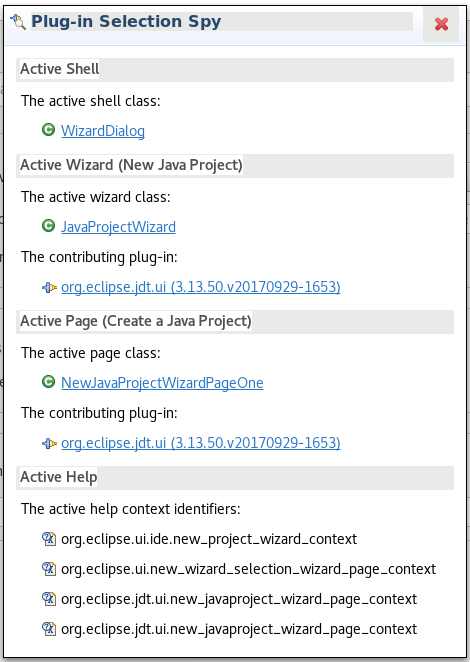
\includegraphics[width=\textwidth,height=0.8\textheight,keepaspectratio]{plugin_spy.png}
\end{center}
\end{frame}

\subsection{Waiting conditions}
\begin{frame}[fragile]
\frametitle{Waiting conditions}
Wait for some time (-Drd.timePeriodFactor)
\begin{lstlisting}
AbstractWait.sleep(TimePeriod.SHORT);
\end{lstlisting}
Wait until/until a condition is met
\begin{lstlisting}
new WaitWhile(new JobIsRunning(), TimePeriod.LONG);
new WaitUntil(new ShellIsAvailable("New Java Project"));
\end{lstlisting}
Not all conditions must be met
\begin{lstlisting}
new WaitUntil(condition, false);
if (condition.getResult() != null) { ... }
\end{lstlisting}
You can also group conditions
\begin{lstlisting}
new GroupWait(TimePeriod.LONG, condition1, condition2, ...);
\end{lstlisting}
\end{frame}

\subsection{Requirements}
\begin{frame}[fragile]
\frametitle{Requirements}
\begin{itemize}
\item Requirements are fulfilled before @BeforeClass
\item By requirements you can set the testing environment
\item Specified by -Drd.config
\item Only yaml and json files are supported
\vspace{0.5cm}
\begin{verbatim}
org.eclipse.reddeer.requirements...ApacheTomcatServer
- runtime": "/tmp/servers/tomcat/apache-tomcat-7.0.82"
  version": "7.0"
\end{verbatim}
\end{itemize}
\end{frame}

\begin{frame}[fragile]
\frametitle{Requirements}
\begin{lstlisting}
@RunWith(RedDeerSuite.class)
@ApacheTomcatServer(state=ServerRequirementState.RUNNING)
public class ServerPresentTest {

  @InjectRequirement
  protected ApacheTomcatServerRequirement requirement;

  @RequirementRestriction
  public static RequirementMatcher getRestrictionMatcher() {
    return new RequirementMatcher(ApacheTomcatServer.class, 
      "version" , new VersionMatcher(">=7.0"));
  }

  ...

}
\end{lstlisting}
\end{frame}

\subsection{Graphiti}
\begin{frame}[fragile]
\begin{center}
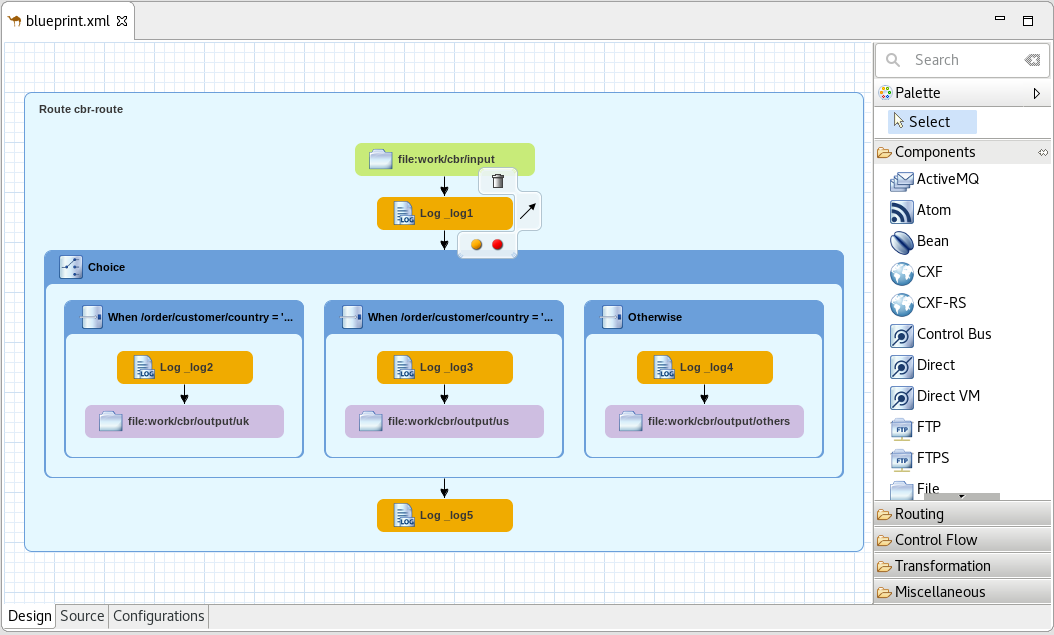
\includegraphics[width=\textwidth,height=0.8\textheight,keepaspectratio]{fuse_tooling.png}
\end{center}
\end{frame}

\begin{frame}[fragile]
\frametitle{Requirements}
\begin{lstlisting}
GEFEditor gefEditor = new GEFEditor("blueprint.xml");
gefEditor.addToolFromPalette("Log", 50, 100);
gefEditor.addToolFromPalette("Bean", 200, 100);

GraphitiEditPart bean = new LabeledGraphitiEditPart("Bean");
bean.select();
bean.getContextButton("Delete").click();

Shell shell = new DefaultShell("Confirm Delete");
new PushButton(shell, "Yes").click();
new WaitWhile(new ShellIsAvailable(shell);
\end{lstlisting}
\end{frame}

\section{Evaluate the session}
\begin{frame}[fragile]
\begin{center}

\includegraphics[width=\textwidth,height=0.8\textheight,keepaspectratio]{SpeakerEvalSlide-16-9-2017.png}
\end{center}
\end{frame}

\end{document}
